\documentclass[]{article}
\usepackage{amssymb}
\usepackage{amsmath}
\usepackage[utf8]{inputenc}
\usepackage{graphicx}
\usepackage{booktabs}
\usepackage{listings}
\usepackage{color}
\usepackage{tabularx}
\usepackage{hyperref}

\definecolor{dkgreen}{rgb}{0,0.6,0}
\definecolor{gray}{rgb}{0.5,0.5,0.5}
\definecolor{mauve}{rgb}{0.58,0,0.82}

\lstset{frame=tb,
	%language=C++,
	aboveskip=3mm,
	belowskip=3mm,
	showstringspaces=false,
	columns=flexible,
	basicstyle={\small\ttfamily},
	numbers=none,
	numberstyle=\tiny\color{gray},
	keywordstyle=\color{blue},
	commentstyle=\color{dkgreen},
	stringstyle=\color{mauve},
	breaklines=false,
	breakatwhitespace=true,
	tabsize=2
}

\title{Evaluation of the Jacobi and Polynomial expansion eigenvalue algorithms}
\author{Olav Fønstelien}

\begin{document}
\maketitle

\begin{abstract}
%The abstract gives the reader a quick overview of what has been done and the most important results. Try to be to the point and state your main findings.
We will study two algorithms for solving the eigenvalue problem $\mathbf{Au} = \lambda \mathbf{u}$; Jacobi's algorithm and an algorithm by polynomial expansion. We test the algorithms by solving two second order differential equations, first evaluating their correctness with a tridiagonal Toeplitz matrix $\mathbf{A}$, then their overall performance with regards to precision, speed and memory usage on a matrix having non-constant central diagonals. We will see that the Polynomial expansion algorithm exceeds the performance of the Jacobi algorithm on all metrics.
\end{abstract}

\section{Introduction}
%When you write the introduction you could focus on the following aspects
%-Motivate the reader, the first part of the introduction gives always a motivation and tries to give the overarching ideas
%-What I have done
%-The structure of the report, how it is organized etc

This work is my submission for the second project in the course FYS4150 given at University of Oslo, autumn 2020 \cite{fys4150},\cite{fys4150-p2}. Parts a)-d) plus g) have been answered. I have implemented the algorithms in C++ using the Armadillo library. You will find the source code at my repository \url{https://github.com/fonstelien/FYS4150/tree/master/project2}.

We will study two iterative algorithms for numerical solutions to eigenvalue problems $\mathbf{Au} = \lambda \mathbf{u}$ and apply them to second order differential equations with Dirichlet boundary conditions on the form
\begin{equation}
\label{diff_1}
	\frac{d^2 u(\rho)}{d\rho^2} = -\lambda u(\rho),
\end{equation}
and
\begin{equation}
\label{diff_2}
	-\frac{d^2}{d\rho^2} u(\rho) + \rho^2u(\rho)  = \lambda u(\rho).
\end{equation}

The first algorithm is the Jacobi eigenvalue algorithm, and the second is a solution based on iterative expansion of the characteristic polynomial $p(x) = \det(\mathbf{A} - x\mathbf{I})$. I will first introduce the mathematical background, then move over to presenting how the algorithms can be implemented, before I evaluate their performance relative to each other.

\subsection{Mathematical basis for the Jacobi eigenvalue method}
Given the eigenvalue problem $\mathbf{Au} = \lambda \mathbf{u}$ where $\mathbf{A}$ is symmetrical. The Jacobi algorithm aims to diagonalize $\mathbf{A}$ by iterative application of pairwise \textit{Givens rotations}. $\mathbf{A}$ is rotated about an orthogonal matrix $\mathbf{S}$ and its transpose $\mathbf{S}^\intercal$ , such that 
\[
\mathbf{S}^\intercal \mathbf{A} = \lambda \mathbf{S}^\intercal \mathbf{u} \Rightarrow \mathbf{S}^\intercal \mathbf{A} \mathbf{S} (\mathbf{S}^\intercal \mathbf{u})= \lambda \mathbf{S}^\intercal \mathbf{u}.
\]

With $\mathbf{S} = \mathbf{S}_m \mathbf{S}_{m-1} \cdots \mathbf{S}_1$, the $\mathbf{S}_i$s will be chosen such that
\[
\mathbf{S}^\intercal \mathbf{A} \mathbf{S} = \mathbf{D}, 
\]
and hence
\[
\mathbf{D} (\mathbf{S}^\intercal \mathbf{u})= \lambda \mathbf{I} (\mathbf{S}^\intercal \mathbf{u}) \Rightarrow \mathbf{D}_{n \times n} = \mathrm{diag}(\lambda_1, \lambda_2, \ldots, \lambda_n).
\]
See \cite{fys4150-notes}. The \textit{Givens matrices} \cite{mat-inf4130} $\mathbf{S}_i$ are given by
\begin{equation*}
\mathbf{S}_i = \mathbf{S}_{kl}
\begin{bmatrix}
\mathbf{I}_k & \mathbf{0} & \mathbf{0} \\
\mathbf{0} & \mathbf{G}_{l-k}(\theta) & \mathbf{0} \\
\mathbf{0} & \mathbf{0} & \mathbf{I} \\
\end{bmatrix}
\text{, where }
\mathbf{G}_{l-k}(\theta) = 
\begin{bmatrix}
\cos \theta 	& 0 		& \cdots 		& -\sin \theta \\
0 				& 1 		& \ddots 		& 0 \\
\vdots 			& \ddots	& \ddots 		& \vdots \\
\sin \theta 	& 0 		& \cdots 		& \cos \theta \\
\end{bmatrix} \in \mathbb{R}^{(l-k) \times (l-k)}.
\end{equation*}

After the first dual rotation, we obtain $\mathbf{S}_1^\intercal \mathbf{A} \mathbf{S}_1 = \mathbf{B}$, where $\mathbf{B}_i$ is symmetrical with elements
\begin{equation}
\label{b_elements}
\begin{array}{cc}
\left\{
\begin{aligned}
b_{jj} =& a_{jj} \\
b_{jk} =& a_{jk}\cos\theta - a_{jl}\sin\theta \\
b_{jl} =& a_{jl}\cos\theta + a_{jk}\sin\theta \\
b_{kk} =& a_{kk}\cos^2\theta - 2a_{kl}\cos\theta \sin\theta +a_{ll}\sin^2\theta\nonumber\\
b_{ll} =& a_{ll}\cos^2\theta +2a_{kl}\cos\theta \sin\theta +a_{kk}\sin^2\theta\nonumber\\
b_{kl} =& (a_{kk}-a_{ll})\cos\theta \sin\theta +a_{kl}(\cos^2\theta-\sin^2\theta)\nonumber 
\end{aligned}
\right\} &
\text{, where } j \ne k,l.
\end{array}
\end{equation}
As outlined in \cite{fys4150-notes}, choosing $k$ and $l$ such that the Givens matrix targets $\mathbf{A}$'s largest off-diagonal element $a_{kl}$, will move $\mathbf{B}_i$ closer to diagonal form for every iteration. We will therefore choose the angle $\theta$ such that $b_{kl} = b_{lk} = 0$, find $\mathbf{B}_i$'s largest off-diagonal element and repeat the process until it converges for some arbitrary $\varepsilon > \max_{k \neq l} \mathbf{B}_i$.

With $\mathbf{v} = \mathbf{S}^\intercal \mathbf{u}$ and $\mathbf{D} \mathbf{v} = \lambda \mathbf{v}$ we see that the transformation preserves $\mathbf{A}$'s eigenvalues such that $\mathbf{D}$ is \textit{similar} to $\mathbf{A}$, but that $\mathbf{D}$'s eigenvectors $\mathbf{v}$ are rotated by $\mathbf{S}^\intercal$ relative to $\mathbf{A}$'s. However, the transformation preserves the dot product and orthogonality:
\[
\mathbf{v}^\intercal \mathbf{v} = (\mathbf{S}^\intercal \mathbf{u})^\intercal (\mathbf{S}^\intercal \mathbf{u}) = \mathbf{u}^\intercal (\mathbf{S} \mathbf{S}^\intercal) \mathbf{u} = \mathbf{u}^\intercal \mathbf{u}.
\]
Since $\mathbf{A}$ is symmetric, its eigenvectors $\mathbf{u} = [\mathbf{u}_1 \quad \mathbf{u}_2\ldots ]$ are orthogonal and therefore, assuming normalization, we have that
\[
\mathbf{v}^\intercal_i \mathbf{v}_j = \mathbf{u}^\intercal_i \mathbf{u}_j = \delta_{ij},
\]
where $\delta_{ij}$ is the \textit{Kronecker delta}.


\subsection{Mathematical basis for the Polynomial expansion method}
A solution to the eigenvalue problem $\mathbf{Au} = \lambda \mathbf{u}$, with $\mathbf{A} \in \mathbb{R}^{n \times n}$, can always be obtained by solving 
\begin{equation}
\label{char_pol}
p(x) = \det(\mathbf{A} - x\mathbf{I}) = 0,
\end{equation}
where $p(x)$ is the characteristic polynomial. However, for arbitrary $n$, an analytic solution to (\ref{char_pol}) may not always be possible \cite{fys4150-notes}. A numerical approximation is therefore necessary. From \textit{Gerschgorin's circle theorem} \cite{mat-inf4130} we know in what area the eigenvalues of matrix $\mathbf{A}$ lies in:
\[
|\lambda - a_{ii}| \leq \sum_{\substack{j=1 \\ j \neq i}}^{n} |a_{ij}|.
\]
The direct approach would therefore be search all rows $i$ and to establish the limits $[x_{min}, x_{max}]$, and to iterate over this range with some step length $h$. However, as shown in \cite{mat-inf4130}, we also know that if $\mathbf{A} \in \mathbb{R}^{n \times n}$ is irreducible, tridiagonal and symmetric, the roots of $p_k(x) = \det(\mathbf{A}_k - x\mathbf{I}_k)$, where $\mathbf{A}_k$ is the upper left $k \times k$ corner of $\mathbf{A}$, are arranged such that they separate the roots of $p_{k+1}(x)$:
\[
\lambda_i^{(k+1)} < \lambda_i^{(k)} < \lambda_{i+1}^{(k+1)}.
\]

Hence, with an iterative approach where we increment $k$, we will be able to narrow down the area to search for each of the roots of $p(x)$ (\ref{char_pol}).

\section{Methods}
%-Describe the methods and algorithms
%-You need to explain how you implemented the methods and also say something about the structure of your algorithm and present some parts of your code
%-You should plug in some calculations to demonstrate your code, such as selected runs used to validate and verify your results. The latter is extremely important!! A reader needs to understand that your code reproduces selected benchmarks and reproduces previous results, either numerical and/or well-known closed form expressions.

\subsection{Jacobi eigenvalue algorithm}
As we stated above, if $\mathbf{A}$ is symmetrical and $\mathbf{S}_1$ is a Givens matrix, $\mathbf{S}_1^\intercal \mathbf{A} \mathbf{S}_1 = \mathbf{B}$  $\mathbf{B}_i$, where $\mathbf{A}$ is symmetrical. Following \cite{fys4150-p2} we can set $s = \sin \theta$, $s = \cos \theta$, $t = s/c$, and rewrite the results from (\ref{b_elements}) such that
\begin{equation}
\label{b_elements_new}
\begin{array}{cc}
\left\{
\begin{aligned}
b_{jj} =& a_{jj} \\
b_{jk} =& a_{jk}c - a_{jl}s \\
b_{jl} =& a_{jl}c + a_{jk}s \\
b_{kk} =& a_{kk}c^2 - 2a_{kl}cs +a_{ll}s^2 \\
b_{ll} =& a_{ll}c^2\theta +2a_{kl}cs +a_{kk}s^2 \\
b_{kl} =& 0 
\end{aligned}
\right\} &
\text{, where } j \ne k,l.
\end{array}
\end{equation}
$b_{kl} = 0$ is achieved by letting
\[
	(a_{kk}-a_{ll})cs +a_{kl}(c^2-s^2) = 0 \Rightarrow -t^2 + \frac{a_{kk}-a_{ll}}{a_{kl}}t + 1 = 0.
\]
Now, with $\tau = \frac{a_{kk}-a_{ll}}{2a_{kl}}$, we get the roots $t = -\tau \pm \sqrt{\tau^2 + 1}$. For numerical stability, we must be careful to pick the right root:
\begin{equation*}
\begin{aligned}
	t_{\tau<0} =& \frac{1}{|\tau| + \sqrt{\tau^2 + 1}} \\
	t_{\tau \ge 0} =& \frac{1}{-\tau - \sqrt{\tau^2 + 1}}
\end{aligned},
\end{equation*}
and at last we can update the $\mathbf{B}$'s elements in (\ref{b_elements_new}) with $c = 1/\sqrt{t^2 + 1}$ and $s = tc$. Here we also see the algorithm's greatest weakness, that it will set elements that it earlier had put to zer, to some non-zero value, meaning that the process potentially has to be repeated for the same element again later in the process.

A possible implementation is outlined in Listing \ref{lst:jacobi} below. The Jacobi algorithm runs in $\mathcal{O}(n^3)$ time, and converges typically after $12n^3$ to $20n^3$ operations \cite{fys4150-notes}, depending on $\mathbf{A}$ and our choice of tolerance $\varepsilon > \max_{k \neq l} \mathbf{B}_i$.

To verify the algorithm we will apply it on the problem in (\ref{diff_1}), which has a tridiagonal Toeplitz representation 
\begin{equation}
\label{toeplitz_matrix}
\mathbf{A} = 
\frac{1}{h^2}
\begin{bmatrix}
2		& -1			& 0				& \cdots 	& 0 \\
-1		& \ddots		& \ddots		& \ddots 	& \vdots \\
0		& \ddots		& 				& 		 	& \\
\vdots	& \ddots		& 				& 		 	& -1 \\
0		& \cdots		& 				& -1 		& 2 \\

\end{bmatrix}
\end{equation}
where $h = 1.0/n$. See \cite{fys4150-p2} for outline. With $\varepsilon = 1.0 \cdot 10^{-2}$, the algorithm performs 113 rotations on a $10 \times 10$ matrix and gives very good precision even if the tolerance is not too strict, as we see in Table \ref{tab:toeplitz_methods} below.
\begin{table}[ht]
	\caption{Results from running the Jacobi eigenvalue algorithm on a $10 \times 10$ Toeplitz matrix with tolerance $\varepsilon = 1.0 \cdot 10^{-2}$. The precision is very high, around 7-8 leading digits, even for relatively high $\varepsilon$. The algorithm ran 113 times before it converged.}
	\label{tab:toeplitz_methods}
	\begin{center}
		\begin{tabular}{lll}
			\toprule
			$\lambda_i$ &              exact &            numeric \\
			\midrule
				0 & 8.1014052771e+00 & 8.1014062027e+00 \\
				1 & 3.1749293434e+01 & 3.1749318745e+01 \\
				2 & 6.9027853211e+01 & 6.9027858255e+01 \\
				3 & 1.1691699740e+02 & 1.1691701506e+02 \\
				4 & 1.7153703235e+02 & 1.7153703274e+02 \\
				5 & 2.2846296765e+02 & 2.2846301971e+02 \\
				6 & 2.8308300260e+02 & 2.8308304077e+02 \\
				7 & 3.3097214679e+02 & 3.3097216033e+02 \\
				8 & 3.6825070657e+02 & 3.6825073262e+02 \\
				9 & 3.9189859472e+02 & 3.9189859742e+02 \\
			\bottomrule
		\end{tabular}
	\end{center}
\end{table}

\begin{lstlisting}[caption={Jacobi eigenvalue algorithm},label={lst:jacobi}]
A = Symmetric NxN matrix
k,l = row, col indexes
eps = tolerance for convergence

k,l = MAX(A)  \\ Finds max element in A and returns row, col indexes

\\ Rotating
WHILE A(k,l) > eps DO 
	\\ Finding the right rotation
	a_kk = A(k,k)
	a_kl = A(k,l)
	a_ll = A(l,l)

	tau = (a_ll - a_kk) / (2*a_kl)
	IF (tau > 0)
		t = 1/(tau + sqrt(tau^2 + 1))
	ELSE
		t = 1/(tau - sqrt(tau^2 + 1))
	END IF
	
	c = 1/SQRT(1 + t^2)
	s = c*t
	
	\\ Updating A
	A(k,k) = a_kk*c^2 - 2*a_kl*s*c + a_ll*s^2
	A(k,l) = A(l,k) = 0.
	A(l,l) = a_ll*c^2 + 2*a_kl*s*c + a_kk*s^2
	
	FOR i = 0 ... N-1 DO
		IF NOT (i == k || i == l)
			a_ik = A(i,k)
			a_il = A(i,l)
			A(i,k) = A(k,i) = a_ik*c - a_il*s
			A(i,l) = A(l,i) = a_il*c + a_ik*s
		END IF
	END DO
	k,l = MAX(A)
END DO

\end{lstlisting}




\subsection{Polynomial expansion algorithm}
We saw above that the roots of $p(x) = \det(\mathbf{A} - x\mathbf{I})$ all lie in the area
\[
|x - a_{ii}| \leq \sum_{\substack{j=1 \\ j \neq i}}^{n} |a_{ij}|.
\]
If we limit our algorithm to positive definite $\mathbf{A}$ (symmetric and diagonally dominant \cite{diagdom}), and that every $k \times k$ sub-matrix $\mathbf{A}_k$ is also positive definite, we can define the limits for where to search for the roots of $p_k(x)$ as
\begin{equation}
\label{poly_limits}
	0 \le x^{(k)} \le \sum_{j=1}^{n} |a_{ij}^{(k)}| \text{;    and    } x_i^{(k+1)} < x_i^{(k)} < x_{i+1}^{(k+1)}.
\end{equation}

Our algorithm will start with $k=2$, whose roots are found directly, then incrementally search for the roots of $p_(k+1)(x)$ within the limits in (\ref{poly_limits}) by bisection. 

A possible implementation for solving the eigenvalue problem in (\ref{diff_1}) with the matrix in (\ref{toeplitz_matrix}) is outlined in Listing \ref{lst:poly_exp_toep} below. As the Jakobi algorithm, the Polynomial expansion algorithm runs in $\mathcal{O}(n^3)$ time.

In routine \lstinline|p(k, x)| we have used the iterative calculation of 
\begin{equation}
\label{pkx}
p_k(x) = (d-x)p_{k-1}(x) - e^2p_{k-2}(x),
\end{equation}
and to avoid overflow, we pull the $1/h^2$ factor in $\mathbf{A}$ (\ref{toeplitz_matrix}) out of the calculations and instead multiply the resulting \lstinline|eigenvals| by this factor to obtain the right answers. However, for the problem in (\ref{diff_2}), where the diagonal elements of $\mathbf{A}$ are on the form $2/h^2 + (ih)^2$, avoiding numerical imprecision and overflow is not possible with the characteristic polynomial on the form that it has in (\ref{pkx}), so we have to divide $p_k(x)$ by $p_{k-1}(x)$ to achieve the numerically better form 
\begin{equation}
\label{qkx}
q_k(x) = (d-x) - e^2/q_{k-1}(x).
\end{equation}
See \cite{barth1967calculation} for further details.

Verification of the algorithm is again done on a $10 \times 10$ matrix, and we see in Table \ref{tab:poly_toeplitz_methods} that it produces good results, with $4$-$6$ leading digits precision for a root search $\varepsilon = 1.0 \cdot 10^{-6}$. For the root search, \lstinline|maxiter| is necessary in case the range does not converge due to numerical imprecision, but does not have to be set very high since the search range is divided by $2$ for every iteration and quickly approaches $0$. In Table \ref{tab:poly_toeplitz_methods} \lstinline|maxiter| was set to 50.

\begin{table}[ht]
	\caption{Results from running the Polynomial expansion eigenvalue algorithm on a $10 \times 10$ Toeplitz matrix with tolerance $\varepsilon = 1.0 \cdot 10^{-6}$ for the root search. Precision is around 4-6 leading digits.}
	\label{tab:poly_toeplitz_methods}
	\begin{center}
		\begin{tabular}{lll}
			\toprule
			$\lambda_i$ &              exact &            numeric \\
			\midrule
				0 & 8.1014053e+00 & 8.1014062e+00 \\
				1 & 3.1749293e+01 & 3.1749319e+01 \\
				2 & 6.9027853e+01 & 6.9027858e+01 \\
				3 & 1.1691700e+02 & 1.1691702e+02 \\
				4 & 1.7153703e+02 & 1.7153703e+02 \\
				5 & 2.2846297e+02 & 2.2846302e+02 \\
				6 & 2.8308300e+02 & 2.8308304e+02 \\
				7 & 3.3097215e+02 & 3.3097216e+02 \\
				8 & 3.6825071e+02 & 3.6825073e+02 \\
				9 & 3.9189859e+02 & 3.9189860e+02 \\
			\bottomrule
		\end{tabular}
	\end{center}
\end{table}


\begin{lstlisting}[caption={Polynomial expansion eigenvalue algorithm for Toeplitz matrix},label={lst:poly_exp_toep}]
N = rows in the A matrix
eigenvals = array of length N

\\ Finding roots by polynomial expansion
eigenvals[0] = d - sqrt(-e);  \\ roots for k=2
eigenvals[1] = d + sqrt(-e);

\\ Finding roots by polynomial expansion
FOR k = 3 ... N-1 DO
	\\ Find the first k-1 roots
	x_min = 0.
	i = 0
	WHILE i < k-1 DO
		x_max = eigenvals[i]
		eigenvals[i] = bisection_root_search(k, x_min, x_max)
		x_min = x_max
		i++
	END DO
	
	\\ find the kth root
	x_min = x_max
	x_max = d + 2*ABS(e)
	eigenvals[i] = bisection_root_search(k, x_min, x_max)
END DO

\\ Avoiding overflow for N > approx. 90
h = 1./N  \\ step length
eigenvals = eigenvals / h^2

\\ Finds the root of pk(x) in the range [x_min, x_max]
ROUTINE bisection_root_search(k, x_min, x_max)
	eps = convergence tolerance
	maxiter = maximum number of iterations
	
	x_left = x_min
	x_right = x_max
	i = 0
	
	WHILE (x_right-x_left)/(x_max-x_min) > eps && i < maxiter DO
		x_mid = (x_right + x_left) / 2
		IF p(k, x_mid) == 0 DO
			RETURN x_mid
		END DO
		
		IF p(k, x_left)*p(k, x_mid) < 0 DO
			x_right = x_mid
		ELSE
			x_left = x_mid
		END DO
	END DO
	
	RETURN x_right
END ROUTINE

\\ Calculates the characteristic polynomial pk(x)
ROUTINE p(k, x)
	\\ NOTE: We have taken out the h^2 factor from d,e to avoid overflow for N > approx. 90
	d = the center diagonal element of A (constant)
	e = the first off-diagonal elements of A (constant)

    pk_2 = d - x
	IF k == 1 DO
		RETURN pk_2
	END DO
	
	pk_1 = (d - x)*pk_2 - e*e
	IF k == 2 DO
		RETURN pk_1
	END DO

	FOR i = 3 ... k DO
		pk = (d - x)*pk_1 - e^2*pk_2
		pk_2 = pk_1
		pk_1 = pk
		i++
	END DO
	
	RETURN pk
END ROUTINE
\end{lstlisting}


\section{Results}
%-Present your results
%-Give a critical discussion of your work and place it in the correct context.
%-Relate your work to other calculations/studies
%-An eventual reader should be able to reproduce your calculations if she/he wants to do so. All input variables should be properly explained.
%-Make sure that figures and tables should contain enough information in their captions, axis labels etc so that an eventual reader can gain a first impression of your work by studying figures and tables only.

% JAKOBI VS POLY
% Compare CPU time for given N with same number of leading digits precision
% Study the results as functions of the number of integration points N and your approximation to ρmax. 

Figure \ref{fig:rotations_for_varying_n} shows how the number of rotations before convergence increases for increasing size of the problem. We see that it increases exponentially. In Figure \ref{fig:eigenvecs} we see how the eigenvector has been rotated in the process.
\begin{figure}[!htb]
	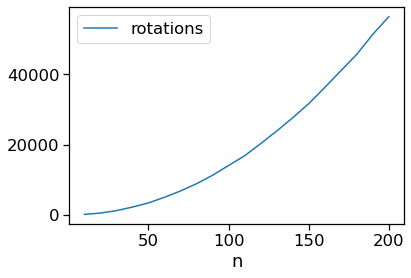
\includegraphics[width=1\linewidth]{./results/rotations_for_varying_n.png}
	\caption{Number of rotations needed for the Jacobi algorithm to converge relative to the size of the problem. $\varepsilon = 1.0 \cdot 10^{-4}$.}
	\label{fig:rotations_for_varying_n}
\end{figure}
\begin{figure}[!htb]
	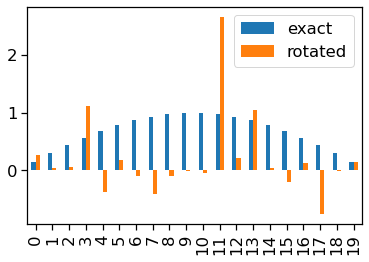
\includegraphics[width=1\linewidth]{./results/eigenvecs.png}
	\caption{The Jacobi algorithm only preserves the eigenvalues. Here we see the original eigenvector $\mathbf{u}$ and the eigenvector after the Givens rotations $\mathbf{S}^\intercal \mathbf{u}$.}
	\label{fig:eigenvecs}
\end{figure}

If we test the Jacobi algorithm on the problem in \ref{diff_2}, where the diagonal elements are given on the form \cite{fys4150-p2} 
\[
a_{ii} = 2/h^2 + (ih)^2
\]
we see that the Jacobi algorithm quickly starts to be too time- and potentially memory-consuming demanding, since the $\mathbf{A}$ matrix must be extended to a large $n$ before we get satisfactory results for the lower eigenvalues. And in contrast to the simple problem with constant diagonal elements, we must also demand a smaller tolerance $\varepsilon$. See Table \ref{tab:jacobi_general}, where a $500 \times 500$ matrix has been solved with tolerance $\varepsilon = 1.0 \cdot 10^{-6}$, and some values for $\rho_{max}$. We see that the precision decreases for growing $\rho_{max}$, as could be expected since the step length $h$ grows. CPU time is more or less constant, depending only on $n$ and $\rho_{max}$.

The Polynomial expansion algorithm performs better for this type of problem. In Table \ref{tab:poly_general} we see that for a similarly conditioned input, we get better precision and a 10-fold increase in performance. However, also here we see that with higher $\rho_{max}$, precision start to be reduced, even if it is less than for the Jacobi method. Here, to avoid numerical overflow, we must calculate the characteristic polynomials using (\ref{qkx}).

\begin{table}[!ht]
	\caption{Results from running the Jacobi eigenvalue algorithm on a $500 \times 500$ matrix with different $\rho_{max}$. Tolerance $\varepsilon = 1.0 \cdot 10^{-6}$. Precision is only 3 leading digits for the lower eigenvalues with, and not usable for th rest. Precision decreases with increasing $\rho_{max}$. CPU time around 70 seconds for all calculations.}
	\label{tab:jacobi_general}
	\begin{center}
		\begin{tabular}{lrlll}
			\toprule
			$\lambda_i$ &              exact &            $\rho_{max} = 4.0$ &            $\rho_{max} = 10.0$ & $\rho_{max} = 20.0$\\
			\midrule
				0   & 3 & 2.982e+00 & 2.955e+00 & 2.910e+00 \\
				1   & 7 & 6.976e+00 & 6.932e+00 & 6.863e+00 \\
				2   & 11 & 1.104e+01 & 1.091e+01 & 1.083e+01 \\
				3   & 15 & 1.554e+01 & 1.490e+01 & 1.479e+01 \\
				4   & 19 & 2.100e+01 & 1.888e+01 & 1.876e+01 \\
				5   & 23 & 2.767e+01 & 2.287e+01 & 2.273e+01 \\
				6   & 27 & 3.560e+01 & 2.686e+01 & 2.670e+01 \\
				7   & 31 & 4.477e+01 & 3.085e+01 & 3.067e+01 \\
				8   & 35 & 5.518e+01 & 3.483e+01 & 3.464e+01 \\
			\bottomrule
		\end{tabular}
	\end{center}
\end{table}

\begin{table}[!ht]
	\caption{Results from running the Polynomial expansion eigenvalue algorithm on a $500 \times 500$ matrix with various $\rho_{max}$. Tolerance $\varepsilon = 1.0 \cdot 10^{-6}$. Precision is up to 5 leading digits for the lower eigenvalues and lower $\rho_{max}$, but, as for Jacobi, the results are not usable for the rest. CPU time about 8 seconds for all calculations.}
	\label{tab:poly_general}
	\begin{center}
		\begin{tabular}{lrlllll}
			\toprule
	$\lambda_i$ &    exact & $\rho_{max} = 4.0$ &  $\rho_{max} = 10.0$ & $\rho_{max} = 20.0$ & $\rho_{max} = 100.0$\\
			\midrule
0   & 3 & 2.999877e+00 & 2.999877e+00 & 2.999503e+00 & 2.987443e+00 \\
1   & 7 & 6.999376e+00 & 6.999376e+00 & 6.997501e+00 & 6.936919e+00 \\
2   & 11 & 1.099848e+01 & 1.099848e+01 & 1.099390e+01 & 1.084529e+01 \\
3   & 15 & 1.499717e+01 & 1.499717e+01 & 1.498869e+01 & 1.471188e+01 \\
4   & 19 & 1.899548e+01 & 1.899548e+01 & 1.898188e+01 & 1.853599e+01 \\
5   & 23 & 2.299338e+01 & 2.299338e+01 & 2.297347e+01 & 2.231685e+01 \\
6   & 27 & 2.699087e+01 & 2.699087e+01 & 2.696345e+01 & 2.605366e+01 \\
7   & 31 & 3.098797e+01 & 3.098797e+01 & 3.095183e+01 & 2.974558e+01 \\
8   & 35 & 3.498467e+01 & 3.498467e+01 & 3.493859e+01 & 3.339169e+01 \\
			\bottomrule
		\end{tabular}
	\end{center}
\end{table}


\section{Conclusion}
%-State your main findings and interpretations
%-Try as far as possible to present perspectives for future work
%-Try to discuss the pros and cons of the methods and possible improvements
Our main findings are that the Jacobi eigenvalue algorithm performs well on solving the eigenvalue problem for Toeplitz matrices, since we can accept a large convergence constant $\varepsilon$ for the off-diagonal elements, but not so well for the more general case where we must increase $n$ in order to give a proper representation of the problem. The value of the diagonal elements increase by $(ih)^2$, meaning that the addition and subtraction of diagonal elements in (\ref{b_elements}) is a source for numerical imprecision, which is accumulated due to the high number of rotations needed, which grow by $\mathcal{O}(n^2)$ \cite{fys4150-notes}.

The Polynomial expansion algorithm performs better, both with regards to time and memory use, and since over/underflow problems can be largely mitigated by calculating the characteristic polynomial with $q_k(x) = (d-x) - e^2/q_{k-1}(x)$, this algorithm is the overall better between the two, and may be the only feasible for problems of size over $n = 10^4$ to $10^5$, due to its memory economy.

\bibliographystyle{plain}
\bibliography{project2.bib}

\end{document}
